%========================================
\chapter{METHODOLOGY}
\label{ch:meth}
%========================================

This chapter presents in the next section the methodology employed in former work, related for the application of a PINN to the solving of the 1D Burgers Equation, including the associated problem of parameter discovery. The following section presents a teste case that uses a DNN implementation to replace the numerical implementation of the gas-optical scheme that is part of the ecRad radiation module of the IFS model used in the ECMWF.

%========================================
\section{PINN Implementation for the 1D Burgers Equation}
%========================================

In former work related to the application of a PINN related to the 1D Buergers equation, three problems were proposed: the use of PINN for the solution of the 1D Burgers' Equation, the discovery of PDE parameters using PINN, and the discovery of PDE parameters using NM.

The problems require data-driven parameter discovery for a given 1D Burgers' Equation, which estimates the velocity field $u$ of a fluid along the dimension $x$ and over time $t$ (\autoref{eq:burg}). In this equation, two coefficients of the differential operators are defined as the parameters $\lambda_1$ and $\lambda_2$. The latter is the kinematic viscosity of the fluid ($\nu$), and the velocity ($u$) subscripts denote partial differentiation in time and space, respectively, as $u_t$ (${du}/{dt}$), $u_x$ (${du}/{dx}$), and $u_{xx}$ (${d^2u}/{dx^2}$).

\begin{equation} \label{eq:burg}
u_t + \lambda_1 u u_x - \lambda_2 u_{xx} = 0
\end{equation}

\noindent In the considered problem, the Burgers' Equation spatial and time domain, and the initial (IC) and boundary conditions (BC), are:
\begin{flalign}
& x \in [-1,1], \ t \in [0, 1], &  \text{(domain)} \nonumber & \\
& u(0, x) = - \sin(\pi x), & 
\text{(IC)} \nonumber & \\
& u(t, -1) = u(t, 1) = 0.  & 
\text{(BC)} \nonumber &
\end{flalign}

Two sets of parameters were used, both using $\lambda_1 = 1$, but with $\lambda_2 = {0.01}/{\pi}$ (expressing low viscosity) for the first, and $\lambda_2 = {0.1}/{\pi}$ for the second (high or usual viscosity). It is intended to demonstrate that small viscosity values in the Burgers' equation can cause discontinuities, which are interpreted as shock waves, and which become more pronounced as the viscosity value decreases, thus making modeling using standard NMs more difficult as it requires more precise spatial and temporal resolutions. In any case, some datasets were generated for the PINN and NM implementations with problem size (dimension $x$ by time $t$) 128x64, 256x100, 256x128, and 512x256 (some were used in specific cases). The datasets were generated using the numerical GQM, which is an iterative numerical algorithm that approximates the definite integral of a function as a weighted sum of the functions values at specified points of the integration domain \cite{Burkardt2013}. The method takes into account the domain, initial and boundary conditions shown above for generating the dataset. The dataset contains the spatial values $x$, the time values $t$, and the exact solution $u(t,x)$.


%========================================
\subsection{PINN Implementation}
%========================================

A part of the code implemented in this work was adapted from \citeonline{Raissi2019}, as described ahead in this work, using Python 3.7 and the framework TensorFlow 1.15 for execution on GPUs. The PINN code is based on an MLP, with an input layer of 2 neurons, a number of hidden layers ranging from 1 to 8, each one with  a number of neurons ranging from 10 to 30, and an output layer with a single neuron. The loss function is based on Mean Squared Error (MSE), and is detailed in \autoref{sec:ppd}. Minimization of the loss function is performed by an optimization method, the generalized Limited-memory Broyden-Fletcher-Goldfarb-Shanno (L-BFGS) algorithm, a quasi-Newton method. All hidden layers employ the hyperbolic tangent as the activation function. 

\begin{minipage}[htb]{\columnwidth}
\begin{lstlisting}[language=Python, label=lst:utx, 
caption={Snippet of Python code that implements $u(t,x)$, seen in the listing as \texttt{net\_u(t, x)}.}]
def neural_net(X, weights, biases):
	num_layers = len(weights) + 1
	H = 2.0 * (X - lb) / (ub - lb) - 1.0
	for l in range(0, num_layers - 2):
		W = weights[l]
		b = biases[l]
		H = tf.tanh(tf.add(tf.matmul(H, W), b))
	W = weights[-1]
	b = biases[-1]
	Y = tf.add(tf.matmul(H, W), b)
	return Y

def net_u(t, x):
	u = neural_net(tf.concat([x, t], 1), weights, biases)
	return u
\end{lstlisting}
\end{minipage}%

The implemented DNN MLP uses the L-BFGS optimizer provided by the SciPy\footnote{\url{https://docs.scipy.org/doc/scipy/reference/Optimize .minimize-bfgs.html}} framework, which was configured to a maximum of 50,000 iterations (a value commonly used by SciPy for such optimizer) and also to stop iterations when the hardware floating point precision lower limit is reached, in this case IEEE-75432 single precision binary floating point. The batch size used is the same size as the CP set, which results in one iteration per training epoch. Some code snippets extracted from the implementation are shown in the Listings \ref{lst:utx}, \ref{lst:ftx}, and \ref{lst:loss}.

\begin{minipage}[htb]{\columnwidth}
\begin{lstlisting}[language=Python, label=lst:ftx, 
caption={Snippet of Python code that implements $f(t,x)$, seen in the listing as \texttt{net\_f(x, t)}. The \texttt{net\_u} function is shown in \autoref{lst:utx}. The \texttt{tf.gradients} is part of the TensorFlow framework and is used in the gradient-based training and optimization algorithm.}]
def net_f(x, t):
	lambda_1 = lambda_1
	lambda_2 = tf.exp(lambda_2)
	u = net_u(t, x)
	u_t = tf.gradients(u, t)[0]
	u_x = tf.gradients(u, x)[0]
	u_xx = tf.gradients(u_x, x)[0]
	f = u_t + lambda_1 * u * u_x - lambda_2 * u_xx
	return f
\end{lstlisting}
\end{minipage}%

\begin{minipage}[htb]{\columnwidth}
\begin{lstlisting}[language=Python, label=lst:loss, 
caption={Snippet of Python code that implements the loss function (\texttt{loss}). The \texttt{u} is the exact solution. The \texttt{net\_u} function is shown in \autoref{lst:utx}. The \texttt{net\_f} function is shown in \autoref{lst:ftx}.}]
u_tf = u  # exact solution
u_pred = net_u(t, x)  # predicted solution using the DNN
f_pred = net_f(t, x)  # predicted solution using the PDE
loss = (tf.reduce_mean(tf.square(u_tf - u_pred)) +
             tf.reduce_mean(tf.square(f_pred)))
\end{lstlisting}
\end{minipage}%

As already mentioned, in the proposed approach, in a first step, the PINN is trained to obtain the parameters of the differential operators, and then the resulting PINN model, which incorporates these parameters, is used to generate a 1D velocity field in the space domain and of time, which will be compared with the exact 1D field generated by GQM.

%========================================
\subsection{PINN Parameter Discovery}
\label{sec:ppd}
%========================================

The PINN training dataset is provided by a set of CPs that were randomly selected from the exact dataset generated by the GQM, for the considered domain and time interval. For a given training iteration $k$, the value of the loss function to be minimized is given by the sum of two Mean Square Errors (MSE),
$MSE_u$ and $MSE_f$ (\autoref{eq:mse}), which can be seen in \autoref{fig:nn}, and the implementation is related to the code snippet in the \autoref{lst:loss}.

The $MSE_{u}$ represents how well the PINN output matches the exact data points of the solution for the set of CPs. It is calculated as the mean squared error of the difference between the exact solution and the PINN predicted output for each CP of the set. In the equation, $N$ is the number of CPs, the term $[u(t^i_u, x^i_u)]$ refers to the exact solution for each CP, and the term [$u^i$] refers to if the solution predicted by DNN, thus the difference $[u(t^i_u, x^i_u)-u^i]$ measures the prediction error. The $MSE_{u}$ can be seen in the \autoref{fig:nn} and in the \autoref{lst:utx}.

The $MSE_f$ represents how well the automatically calculated derivatives  match the actual PDE terms at the CPs within the domain. The mean squared error of the physics-based regularization term ($[f(t^i_u, x^i_u)]$) enforces the compliance to the governing physical equations or constraints.
It can be seen in the \autoref{fig:nn} and in the code snippet shown in the \autoref{lst:ftx}.

The MSE is used in the gradient descent optimization algorithm. The algorithm includes derivatives and automatic differentiation \cite{Baydin2018} to calculate the gradient\footnote{\url{https://www.tensorflow.org /versions/r1.15/api_docs/python/tf/gradients}} of the error function with respect to the parameters of the PINN, to update the network weights and biases at each iteration. The gradient provides guidance to adjust the parameters in value and direction in order to minimize the error.

\begin{equation}
f := u_t + \lambda_1 u u_x - \lambda_2 u_{xx}
\label{eq:ftx}
\end{equation}

\begin{minipage}[htb]{.95\columnwidth}\bigskip\begin{equation}
MSE^k = MSE_u^k + MSE_f^{k-1}
\label{eq:mse}\end{equation}
where
$$ MSE_u^k = \frac{1}{N}\sum_{i=1}^{N}|u(t^i_u, x^i_u)-u^i|^2 $$
and
$$ MSE_f^{k-1} = \frac{1}{N}\sum_{i=1}^{N}|f(t^i_u, x^i_u)|^2 $$
\bigskip\end{minipage}%

\begin{figure}[htb]\centering
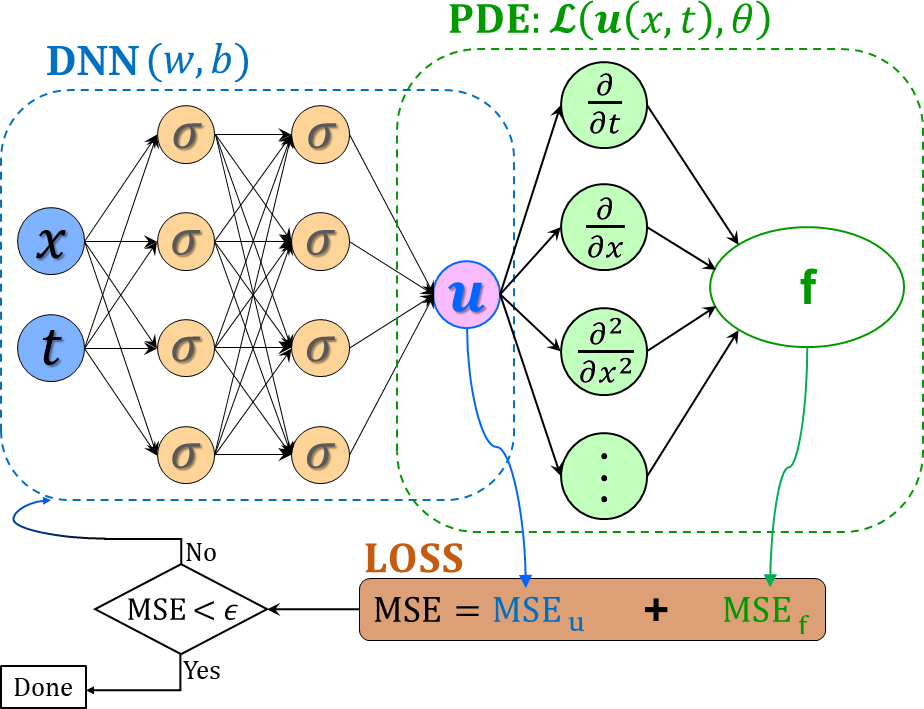
\includegraphics[width=.8\columnwidth]{nn}
\caption{Schematic showing an example structure and loss function, for the PINN approach. The symbol $\theta$ represents the optimization algorithm. The $\epsilon$ represents the smallest threshold error in the optimization algorithm.\\
Source: Adapted from \citeonline{Meng2020}.}
\label{fig:nn}
\end{figure}

According to the work of \citeonline{Raissi2019}, the standard division of the CP dataset into training, validation and testing is not used in this specific PINN model. Instead, a random sample of CPs from the dataset is taken and used to train the PINN. During training, a specific validation set is not used. After training, the network is used to generate two results: ($i$) the discovery of the PDE parameters, and ($ii$) a prediction of the PDE solution.

Once the parameters have been discovered, in a second step, the resulting PINN model is used to predict the velocity field for all points in the defined space and time domain. This predicted velocity field can then be compared with the exact velocity field (generated by GQM), using a relative error to evaluate the accuracy of the prediction, as suggested in Xu et al. (2022) \cite{Xu2022}. Such a relative error is defined by \autoref{eq:error}.

\begin{equation}
R_{L2} = \frac{\| \widehat{U} - U \|}{\|U\|}
\label{eq:error}
\end{equation}

The $\|U\|$ represents the Euclidean L2 norm, which is given by the Euclidean distance from the vector coordinate to the origin of the vector space, i.e. it is the square root of the sum of the squared components of the vector. In the one-dimensional case, the L2 norm is simply given by the value of the velocity.
The $\| \widehat{U} - {U} \| $ represents the application of the L2 norm to the deviation of the estimated velocity field $\widehat{U}$, with respect to the exact velocity field $U$, considering all dataset points in the space and time domains.

The PINN hyperparameters, like the number of hidden layers $N_l(l = 1, 2, ...)$, and the number of neurons in each layer $N_{le}(e = 1, 2, ...)$, can also be optimized by numerical experimentation (trial and error). Optimization of $N_l$ and $N_{le}$, and eventually of other hyperparameters not employed here, is still an unsolved problem, being made empirically \cite{Xu2022}.

As any neural network, PINNs are subjected to overfitting or underfitting. Overfitting means that the DNN performs very well using the training set, but lacks performance using different, new input data of the test set, i.e. it does not generalize. On the other hand, underfitting means that the model performs poorly on both the training and test sets. Obviously, both overfitting and underfitting imply in poor performance of the neural network \cite{Koehrsen2018}.

%========================================
\subsection{NM-based Parameter Discovery}
\label{sec:npd}
%========================================

The inverse problem solved by the implemented PINN to find the coefficients of the differential operators is then compared to the chosen NM-based method, the Sparse Identification of Nonlinear Dynamical Systems (SINDy) method \cite{Boninsegna2018}. This is a method developed for solving the identification problem of dynamical systems, which are systems that change over time. SINDy uses sparse regression to create a linear combination of basis functions to captures the dynamic behavior of the considered physical system. It employs observational or synthetic data to obtain the governing equations that fit such data of the dynamical systems. The discovered equations can then be used to predict future states, inform control inputs, or enable theoretical research using analytical techniques~\cite{Brunton2016}.

Assuming a physical system that evolves in time $t$ and space $x$ defined by a collection of measurements $x(t)\in \mathbb{R}$. Time evolution of $x(t)$ is modeled by SINDy using a nonlinear function $f(x(t))$ (\autoref{eq:sn1}). The vector $x(t)=[x_1(t), x_2(t), \dots x_n(t)]^\top$ represents the state of the physical system at time $t$. The problem solved by SINDy is shown in \autoref{eq:sn2}, where the function $f(x(t))$ is expressed as a matrix $\Theta$ of basis functions applied to the input data $X$, i.e. $\Theta(X)$, which is then multiplied by a matrix $\Xi$ of coefficients that weighs these basis functions. Along the iterations, these coefficients are optimized until achieving convergence by means of an objective function (\autoref{eq:opt}) that assess the correctness of the solution given by [$\Theta(X)\,\Xi$] at a given iteration. It is assumed that $f(x(t))$ is usually sparse in the space of a suitable set of basis functions, i.e. that much of the coefficients of the matrix $\Xi$ are zero. 

\begin{equation}
\frac{d}{dt}x(t) = f(x(t))
\label{eq:sn1}\end{equation}

\begin{equation}
\dot{X} \; = \Theta \,(X)\,\,\Xi
\label{eq:sn2}
\end{equation}

SINDy applies a sparsity-promoting regression (such as LASSO \cite{Tibshirani2011}) to a library of nonlinear candidate functions produced from the measurements, but restricting the number of basis functions to obtain a compact representation of the function and avoid overfitting. SINDy has been effectively used to solve a variety of problems, including linear and nonlinear oscillators, chaotic systems, and fluid dynamics \cite{Brunton2016}. SINDy is implemented by the sparse regression package PySINDy\footnote{\url{http://pysindy.readthedocs.io}} which includes several implementations for the sparse identification method of nonlinear dynamical systems from various authors, being  comprehensive literature reviews available at \cite{DeSilva2020} and \cite{Kaptanoglu2022}. Part of the code implemented in this work was reused and adapted from PySINDy library examples. PySINDy runs on CPU.

This work employs four of these implementations, known as Sparse Regression Optimizers (SRO), which are part of the parameter discovery package and can be selected separately, producing a result for each choice: Sequentially Threshold Least Squares (STLSQ), Orthogonal Least Squares of Forward Regression (FROLS), Sparse Relaxed Regularized Regression (SR3), and Sparse Stepwise Regression (SSR). To keep things simple, we'll treat each of these as a separate NM.

A code snippet of this framework is shown in \autoref{lst:nm}, where \texttt{optimizer} is the chosen optimization method (exemplified in the code as STLSQ), \texttt{SINDy} defines the model, \texttt{fit} discovers the parameters, and \texttt{print} shows the result. 

\begin{minipage}[htb]{\columnwidth}
\begin{lstlisting}[language=Python, label=lst:nm, 
caption={Python code snippet that implements the NM for data-driven PDE parameter discovery. The STLSQ is one of the optimizers in the PySINDy framework.}]
optimizer = ps.STLSQ(threshold=2, alpha=1e-5, normalize_columns=True)
model = ps.SINDy(feature_library=pde_lib,
                 optimizer=optimizer,
                 feature_names=["u"])
model.fit(u, t=dt)
model.print()
\end{lstlisting}
\end{minipage}%

The dataset used by SINDy for each of the 4 optimizers is the same used in the PINN method, but employing the full dataset instead of the set of CPs. Parameter discovery using PINN required training the network with the set of CPs, use of the Burgers' PDE in the loss function, etc. After training, the predicted velocity field in space and time is then compared to the exact field. In the case of SINDy, the complete dataset is used to obtain the parameters, with no further comparison \cite{Brunton2016}. However, parameters discovered by PINN and SINDy are compared in order to evaluate the accuracy of both approaches using the coefficients of the known PDE as reference. Although possible, some optimizations were not made to SINDy in order to obtain better accuracy, being the default settings of the framework used. These possible optimizations can be performed as future work.

Except in the case of SINDy with the SR3 optimizer, the other optimizers employ the objective function that must be minimized, which can be seen in the \autoref{eq:opt}.

\begin{minipage}[htb]{.95\columnwidth}\bigskip\begin{equation}
\| \ y \ - \ X \ w \ \|^2 \ \ + \ \ \alpha \ \| \ w \ \|^2
\label{eq:opt}\end{equation}
Above, $w$ is the weight matrix containing the set of basis functions that maps the dataset contained in $X$ to the solution $y$, i.e. $w$ corresponds to the 2nd member ([$\Theta(X)\,\Xi$]) of \autoref{eq:sn2}, and $\alpha$ is a regularization coefficient applied to $w$, helping prevent overfitting.
\bigskip\end{minipage}%

In order to minimize the objective function, the STLSQ \cite{Brunton2016} algorithm uses ridge regression with sequential threshold, and iteratively runs the least squares algorithm, but masking elements below a specific threshold. The FROLS \cite{Billings2013} algorithm is a greedy algorithm that iteratively selects the most correlated function in the library. The SSR \cite{Boninsegna2018} is also a greedy algorithm that iteratively eliminates the smallest coefficients. A greedy algorithm is any algorithm that uses the heuristic of choosing the locally optimal solution at every iteration \cite{Black2005}. Regardless of not assuredly finding a global optimal solution, greedy heuristics can produce locally optimal solutions that approximate a globally optimal solution in a reasonable amount of time. Along the iterations, the SSR and FROLS algorithms respectively truncate (or add) one nonzero coefficient at each algorithm iteration.

The SR3 algorithm \cite{Champion2019} is a relaxed and sparse regularized regression with linear (dis)equality constraints that attempts to minimize the objective function (\autoref{eq:sr3}).

\begin{minipage}[htb]{.95\columnwidth}\bigskip\begin{equation}\begin{aligned}
&0.5  \|  y  -  X  w \|^2 + \lambda  R(u) + (0.5 / \nu)  \|  w  -  u  \|^2\\
&\text{subject to } Cw = d
\label{eq:sr3}\end{aligned}\end{equation}
over $u$ and $w$, where $R(u)$ is a regularization function, $C$ is a constraint matrix, and $d$ is a vector of values.
\bigskip\end{minipage}%


%========================================
\section{DNN Preliminary Approach for ecRad}
\label{sec:mcw}
%========================================

The problem requires the emulation, using DNN, of the gas-optical algorithm solution of a modern radiation scheme (RTE+RRTMGP), for a wide range of atmospheric conditions, with errors in the heating rates and top-of-atmosphere radiative forcing, typically below $0.1 K day^{-1}$ and $0.5 W m^{-2}$ \cite{Ukkonen2020}.
What is written below is an explanation more linked to the numerical model, but which serves as a basis for emulation. 

Unlike many other phenomena specified in dynamical models, such as clouds and convection, atmospheric radiative transfer is a well-studied issue that can be correctly represented. Modern radiation codes typically use the correlated k approximation and the k-distribution approach to handle the complexity \cite{Goody1989}. The highly variable absorption coefficient spectrum as a function of wavelength, k($\lambda$), is rearranged by $k$ and replaced with a monotonically increasing function $k(g)$, where $g(k)$ is the cumulative distribution function. This function is integrated using a restricted number of quadrature points, referred to as $g$ points. Compared to the line-by-line method, this method significantly reduces the number of monochromatic calculations needed to retrieve fluxes in the SW and LW spectra. 

K-distributions can be applied to an inhomogeneous medium, such as the atmosphere, providing that the mapping of wavelengths to g-space is completely correlated for neighboring atmospheric layers, an approximation that allows fluxes and heating rates to be estimated with less than 1\% uncertainty \cite{Fu1992}. Despite the effectiveness of the correlated k-distribution (CKD) method, radiation calculations in climate models are expensive and performed on a coarser horizontal and temporal grid than others. The ECMWF high-resolution forecast model calls the radiation scheme every 1 hour on a grid with 10.24 times fewer columns than the rest of the model \cite{Hogan2018}.

Because radiation calculations in climate models are expensive, they appear to be a viable area of study for optimizing efficiency without losing accuracy, and one possible approach is the use of PIML.
An interesting aspect about PIML that can be explored in research is the increase in performance of algorithms through the use of single-precision floating-point numbers and the GPU, which is a known feature in algorithms that use DNN.
The preliminary work shows a DNN implementation replacing an existing numerical implementation of the gas-optical scheme (from RRTMGP) of the eCrad model, where performance gains were obtained in preliminary tests, paving the way for future work and a proposal for investigation and implementation of PIML.


%========================================
\subsection{DNN-based Gas Optics Implementation}
\label{sec:mgom}
%========================================

As previously mentioned, the thesis proposes a PIML-based implementation to replace the numerical radiation module ecRad employed in the IFS model of the ECMWF. However, as a preliminary work, a DNN-based model of the RRTMGP gas-optical scheme was implemented for a test case involving a reduced database. The RRTMGP numerical code is part of ecRad module. The accuracy and performance of the DNN implementation were analyzed, taking as reference the corresponding numerical implementation RRTMGP.

The DNN implementation of the gas-optical scheme of the radiation module shown here, the original numerical code (RRTMGP) was replaced by a DNN model. The kernel of the original RRTMGP scheme was written in Fortran 90, and performs a 3D linear interpolation of the optical depth of the atmosphere for the considered 2D grid point using a lookup table indexing temperatures, pressures and mixing fractions. RRTMGP stand for Rapid Radiative Transfer Model for General circulation model (GCM) applications – Parallel \cite{Pincus2019}. It is based on RRTM-G, the Rapid Radiative Transfer Model for GCM-Parallel applications \cite{Hogan2017}. This is a free and open source package that predicts the optical properties of the gaseous atmosphere, includes the solver of the Radiative Transfer Equation called Radiative Transfer for Energetics (RTE), and is used in (numerical) climate and weather models \cite{Pincus2019}. This scheme, like others, includes SW (shortwave) solar radiation and LW (longwave) thermal radiation solving. It employs a statistical k-distribution model based on advanced spectroscopy and numerous g-points, with 256 within 16 LW bands and 224 within 14 SW bands. The RRTMGP code implemented in this work was adapted from \citeonline{Ukkonen2023}. 

The DNN implementation of the gas-optical scheme was developed in a framework composed of the Python 3.12 and the TensorFlow 2.16 library in order to perform training and validation of a MLP neural network using a known dataset. The resulting trained model is saved to disk to later be used in the DNN implementation in Fortran 90 inserted in the radiation module. This Fortran 90 code can be run on CPU or GPUs using cuBLAS and OpenACC, while TensorFlow uses GPU. In the ecRad radiation module, the DNN code is based on Neural Fortran, being called RRTMGP-NN \citeonline{Curcic2019}. 

The standalone ("offline") version of ecRad used in this work is modular, runs on a Unix-like platform, operates independently, and allows investigations and research related to cloud radiative effects without being tied to the operational forecasting model.  It has four components: Gas Optics, Aerosol Optics, Cloud Optics, and Solver. ecRad offers several solvers, including McICA (Monte-Carlo Independent Column Approximation), Tripleclouds, and SPARTACUS \cite{Ukkonen2023}. There is a test version for practical test cases that may run on a standard laptop with GPU and minimum RAM, which was employed in this work and had its performance evaluation analyzed with the Gprof tool.

The input data to the DNN are the temperature, pressure and concentrations of each gas represented in the RRTMGP and, excluding oxygen and nitrogen which are assumed to be constant, this results in 18 LW and 7 SW inputs. In order to predict absorption and Rayleigh optical depths in SW and Planck and absorption optical depths in LW, different models are trained. These are multi-output DNNs that predict all g-points simultaneously, with output sizes of 256 LW or 224 SW. 
In the main code, written in Fortran, the originally numerical gas-optical implementation is replaced by the DNN implementation, also written in Fortran, which uses trained models saved on disk.
The training of the DNN network to obtain the prediction model is implemented in Python using the TensorFlow library, and the final trained model is saved to disk for later use by the Fortran implementation of the main code.
The MLP architectures (layers and neurons) that were used, are described in \autoref{tab:nnmodel}.
In the implementation of the DNN network used in this work, a manual adjustment of the architecture was made, however it would be interesting to use an automated method in future work.
One point that is particularly interesting for the study is that identifying an effective loss function is a significant task, since decreasing the instantaneous imprecision of a specific variable does not guarantee numerical stability over long time intervals, realistic variability, or conservation of energy, moisture, and momentum.

\begin{table}[htb]\centering
\begin{tabular}{cccc}
\hline
     Predicted & Input & 2 Layers & Output \\
\hline
     LW absorption & 18 & 58-58 & 256 \\
     LW emission & 18 & 16-16 & 256 \\
     SW absorption & 7 & 48-48 & 224 \\
     SW scattering & 7 & 16-16 & 224 \\
\hline
\end{tabular}
\vspace{1em}
\caption{Network architectures used for different optical depths.\\
Source: Adapted from \citeonline{Ukkonen2020}.}
\label{tab:nnmodel}
\end{table}

The underlying data flow in a framework of a conventional numerical gas-optical scheme (e.g., RRTMGP) is shown in \autoref{fig:lookup-01}, and the gas-optical scheme it emulates is shown in  \autoref{fig:lookup-02}. In the numerical model, the code calculates the absorption by 1 to 2 major gas species by 3D interpolation in temperature, pressure, and the relative abundance ($\eta$) \cite{Pincus2019}, and contributions from less important gases are computed separately using 2D interpolation, with a given band being written multiple times. In the case of DNN gas optics, all spectral points are predicted simultaneously from an input matrix that includes all gases.

\begin{figure}[htb]\centering
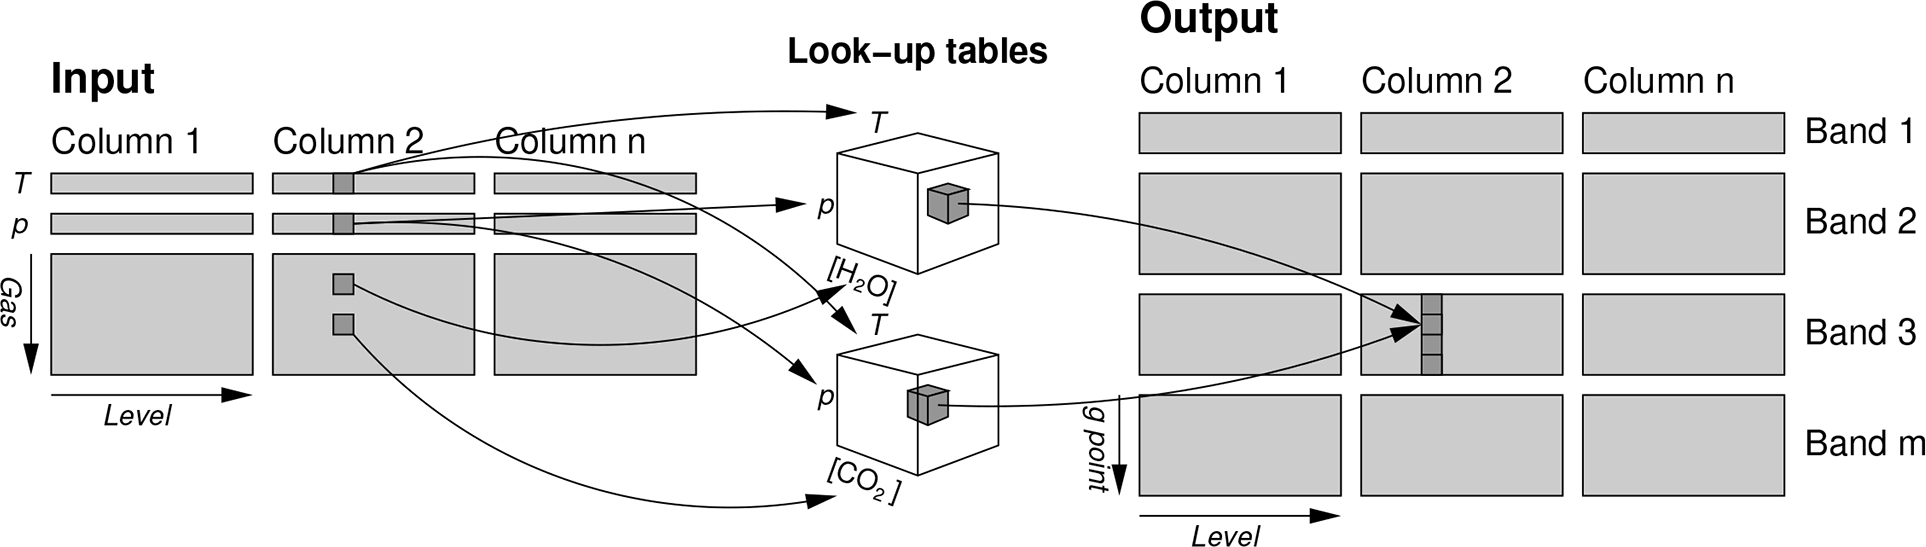
\includegraphics[width=\columnwidth]{lookup-01.png}
\caption{Schematic illustrating the data flow in a structure of a conventional numeric gas optics scheme. "T" is temperature, "p" is pressure, "Gas" represents relative abundance, "Band" corresponds to the LW and SW radiation bands, "g-points" correspond to "k-terms" of the correlated k-distribution method, “Level” corresponds to atmospheric layers or vertical grid points within a column representing altitude or pressure, and "look-up tables" (LUT) correspond to the look-up table kernels of the RRTMGP model. The \autoref{fig:lookup-02} complements this Figure.\\
Source: Adapted from \citeonline{Ukkonen2023}.}
\label{fig:lookup-01}
\end{figure}

\begin{figure}[htb]\centering
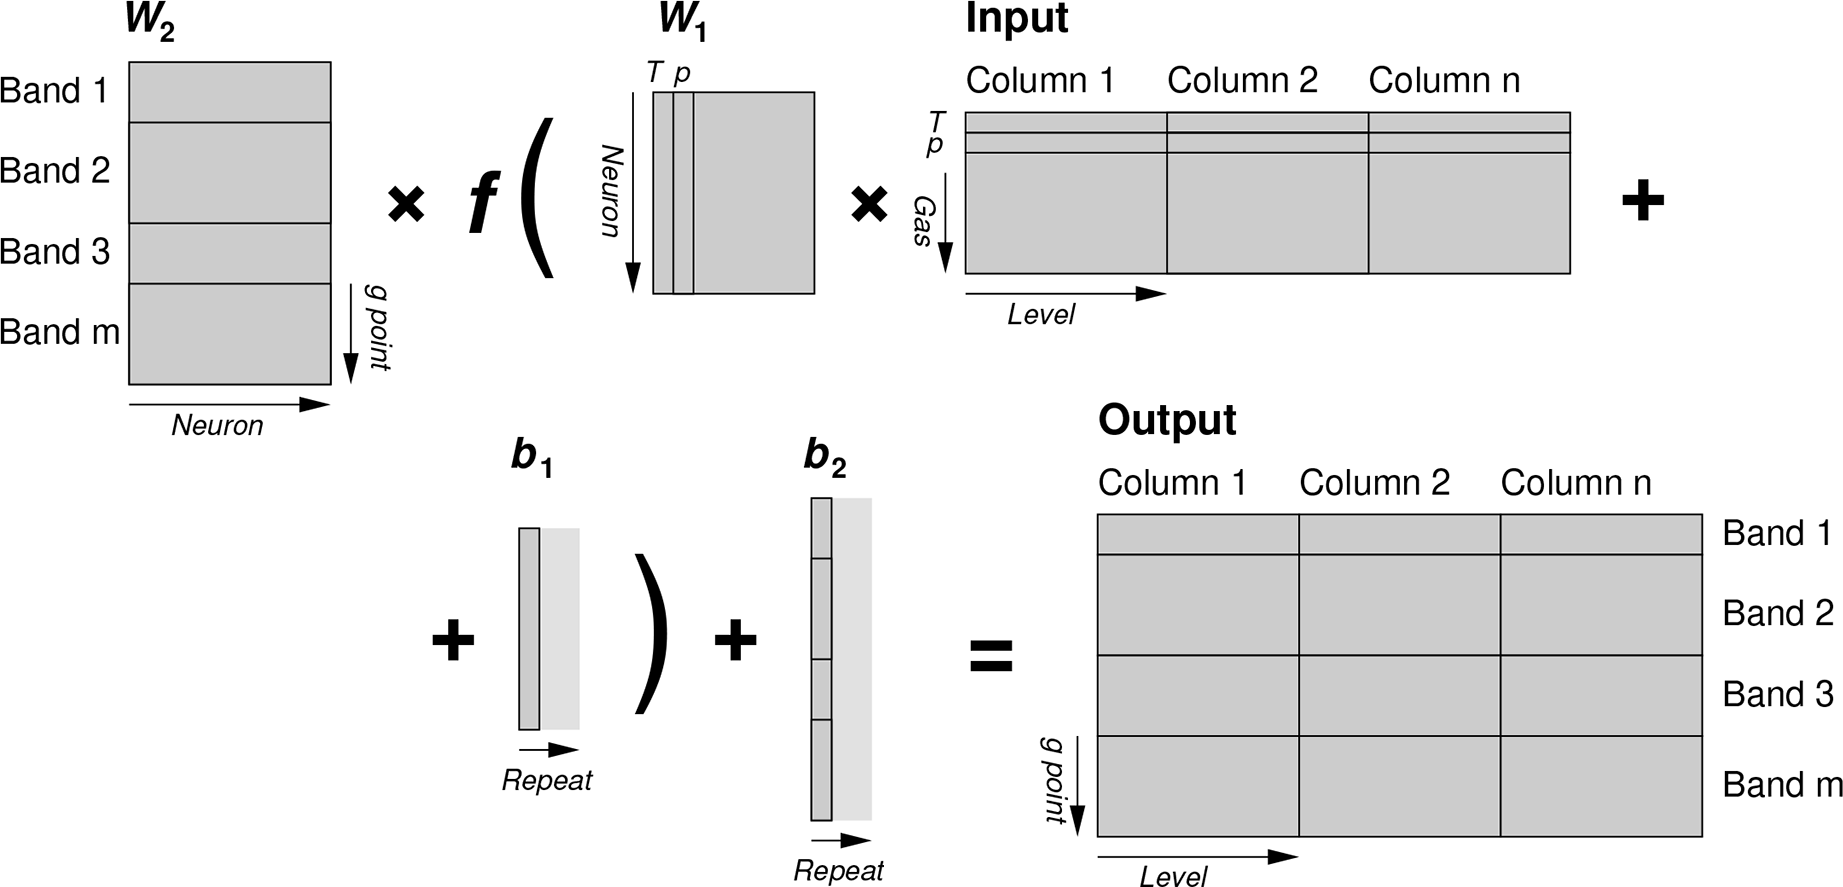
\includegraphics[width=\columnwidth]{lookup-02.png}
\caption{Simplified schematic, with only one hidden layer, illustrating the data flow in a gas optics DNN framework. "W" represents weight, and "b" represents bias. The other terms are described in the \autoref{fig:lookup-01}.\\
Source: Adapted from \citeonline{Ukkonen2023}.}
\label{fig:lookup-02}
\end{figure}

For a given band, vertical level, and column, the RRTMGP calls interpolation kernels several times to compute gas-specific contributions to optical properties, accounting for temperature (T) and pressure (p) dependencies, as well as overlap of major gases in the band. These kernels loop over the g points in a single band, of which there are only 1-12 in the reduced k distributions.

The DNN improves performance by (i) predicting a vector containing all g points from a vector containing T, p, and the mixing ratios of all gases (the DNN implicitly treats gas interactions) and (ii) batching the computations for multiple atmospheric levels and columns by expressing the core DNN computations as matrix-matrix multiplications (between weights W and input matrices) that are delegated to a BLAS library. 

In the chosen DNN loss function (\autoref{eq:ecrnn}), $\alpha$ is a coefficient representing a trade-off between heating rate and radiative forcing errors (e.g. 0.6 for LW and 0.2 for SW), $y$ is the target vector, and $\hat{y}$ is the DNN output vector. It minimizes the error in the difference in y associated with different perturbation experiments as well as the mean squared error of y (scaled DNN outputs) and indirectly measures radiative forcing errors.

\begin{equation}
loss = \alpha \sum_{i=1}^{N}(y_i - \hat{y}_i)^2 + (1 - \alpha)
\sum_{\substack{i=1 \\ i \ \text{odd}}}^{N} ( (y_{i+1} - y_i) - (\hat{y}_{i+1}-\hat{y}_i) )^2
\label{eq:ecrnn}
\end{equation}

The training dataset used is derived from a variety of sources, including existing atmospheric profiles, future climate experiments, and reanalyses, which were synthetically supplemented by varying greenhouse gas concentrations, either manually or using hypercube sampling, as well as data provided by the Radiative Forcing Model Intercomparison Project \cite{Pincus2016}, which includes 100 profiles and 18 perturbations. The profiles were designed to assess global mean clear-sky errors in instantaneous radiative forcing and should be well suited as an out-of-sample test for our purposes, and in addition, a different dataset based on the CAMS reanalysis \cite{Inness2019} is also used that uses the same approach as the IFS and the Correlated k-distribution Model Intercomparison Project (CKDMIP) \cite{Hogan2020}, where only nine gases are considered, but the radiative forcing.

For performance analysis, Gprof was used, which is a performance analysis tool for Unix-based programs, developed as an expanded version of the previous "prof" tool, using a combination of instrumentation and sampling, and which can collect and print a limited number of call graphs. Two analyses were performed, one of the original numerical implementation of ecRad, and another of the version that uses the DNN implementation. The goal was to identify, in a general way, without going into too much detail, the main costly routines.


%========================================
\section{Computing Environment}
\label{sec:cenv}
%========================================

The DNN, PINN and the four PySINDy codes\footnote{The codes are available at \url{http://github.com/efurlanm/pd1b24}} were executed in three different computing environments. It is important to note that the PINN model runs on GPU, DNN runs on CPU/GPU, and PySINDy runs on CPU. The first environment (used in 1D Burgers') is a PC with a 6-core Intel i7-9750H CPU with 6 cores, 8 GB of main memory, and an NVIDIA GTX 1050 GPU (768 CUDA cores and 3 GB of memory). The second (used in DNN RRTMGP) is a PC with 2-core Intel I7-7500U CPU with 2 cores, 16 GB of main memory, and an NVIDIA Geforce 940MX GPU (384 CUDA cores and 4 GB of memory). The third environment (used in DNN RRTMGP) is the Santos Dumont (SDumont) supercomputer of the National Scientific Computing Laboratory (LNCC), more specifically a single Bull Sequana X1120 processing node with two 24-core Intel Xeon Gold 6252 Skylake 2.1 GHz processors (total of 48 cores), 384 GB of main memory and four Nvidia Volta V100 GPUs, although only one GPU was employed. Both computing environments included the Python\footnote{\url{http://www.python.org}} 3.7 interpreter and the TensorFlow\footnote{\url{http://www.tensorflow.org}} v1.15 machine learning platform.

